\begin{figure}[!htbp]
\caption{Volúmenes del pipeline para las tres agrupaciones (MiB)}
\label{fig:volumen_pipeline}
\centering
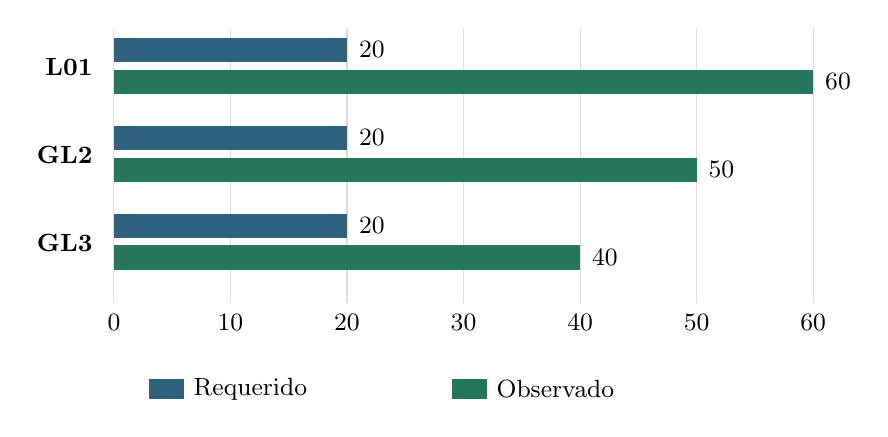
\begin{tikzpicture}[x=0.148cm,y=0.62cm,font=\small]
\definecolor{reqbar}{HTML}{2F627C}
\definecolor{obsbar}{HTML}{26755C}
\foreach \v in {0,10,20,30,40,50,60} {
  \draw[gray!25] (\v,0.18)--(\v,5.8);
  \node[below] at (\v,0.13) {\v};
}
\foreach \y/\caso/\observado in {5/L01/60,3.2/GL2/50,1.4/GL3/40} {
  \node[left,font=\small\bfseries] at (-1,\y) {\caso};
  \fill[reqbar] (0,\y+0.10) rectangle (20,\y+0.60);
  \fill[obsbar] (0,\y-0.55) rectangle (\observado,\y-0.05);
  \node[right] at (20.2,\y+0.36) {20};
  \node[right] at (\observado+0.2,\y-0.30) {\observado};
}
\fill[reqbar] (3,-1.79) rectangle (6,-1.38);
\node[right] at (6,-1.59) {Requerido};
\fill[obsbar] (29,-1.79) rectangle (32,-1.38);
\node[right] at (32,-1.59) {Observado};
\end{tikzpicture}
\end{figure}
